\documentclass[10pt]{article}
\usepackage[utf8]{inputenc}
\usepackage[T1]{fontenc}
\usepackage{graphicx}
\usepackage[export]{adjustbox}
\graphicspath{ {./images/} }
\usepackage{amsmath}
\usepackage{amsfonts}
\usepackage{amssymb}
\usepackage[version=4]{mhchem}
\usepackage{stmaryrd}

\title{SNePS 3 GUI Documentation Version 0.01 Milestone 6 Alpha }

\author{}
\date{}


\begin{document}
\maketitle
May 22, 2010

\begin{center}
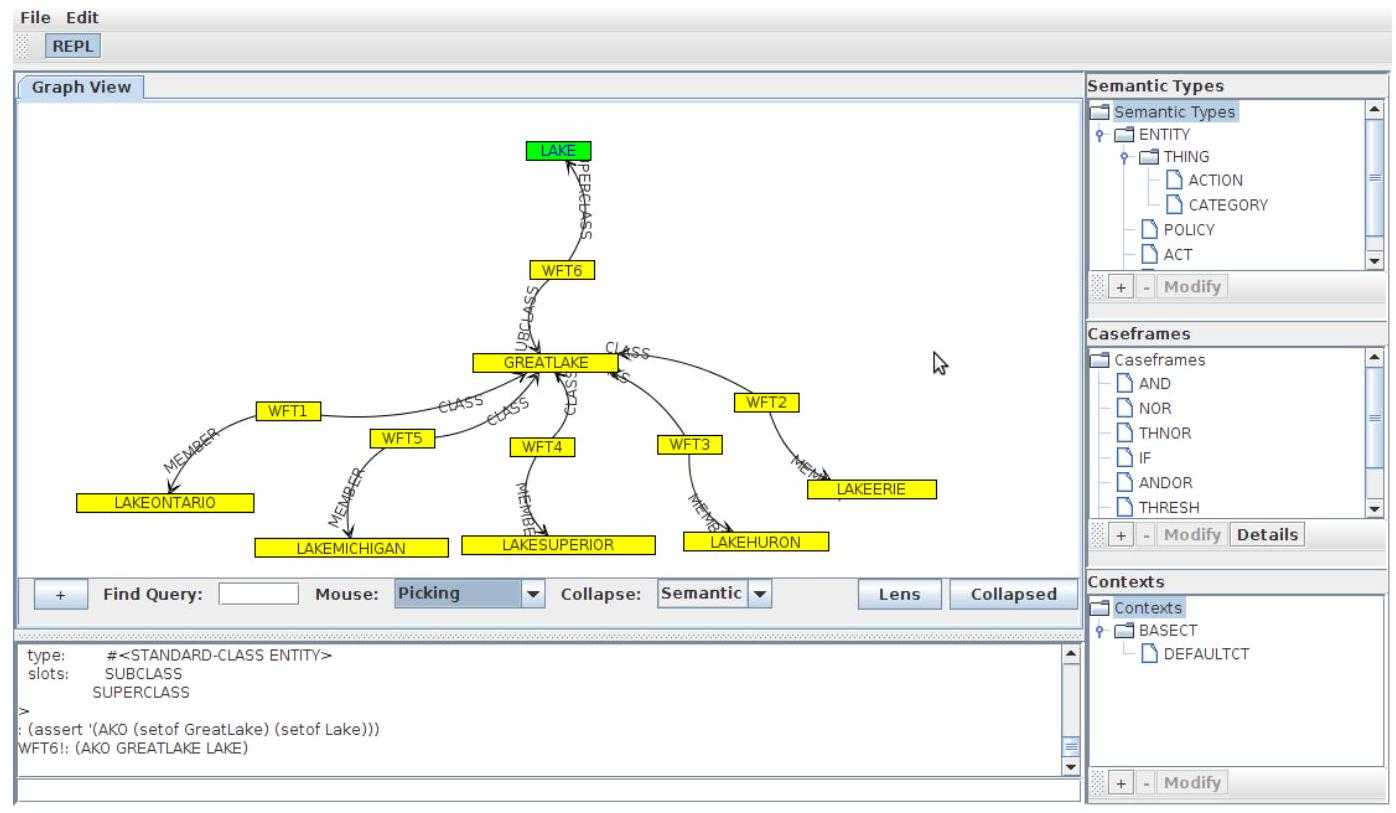
\includegraphics[max width=\textwidth]{2023_06_06_402e2c8ca4c84733095bg-1}
\end{center}

\section{File Operations}
\subsection{Loading a Knowledge Base}
To load a knowledge base, click the File menu, then Load, then "Load to KB." After selecting a file and clicking "Open" the file will be loaded into the SNePS 3 knowledge base. The REPL can be used to view what has been loaded and any feedback from SNePS 3.

\subsection{Loading a Demo}
To load a demo click File $->$ Load $->$ Demo. Select the demo file and click open. The demo window will appear.

\begin{center}
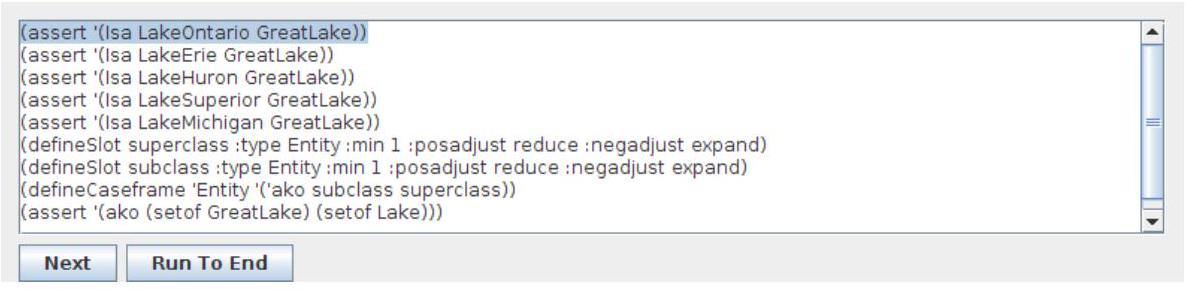
\includegraphics[max width=\textwidth]{2023_06_06_402e2c8ca4c84733095bg-2}
\end{center}

Click Next to execute the next line of the demo, or Run to End to execute the entire demo up to and including the last line.

\subsection{Saving a Knowledge Base}
To save the current knowledge base click File $->$ Save $->$ Current KB. This will save all definitions of semantic types, caseframes, and slots along with all assertions since the last time the knowledge base was cleared.

\subsection{Creating a Demo}
To create a demo you need only follow through the steps you wish to be in the demo, then click File $->$ Save $->$ Demo. This will save the entire contents of the knowledge base since you started.

\subsection{Saving a PNG of the Graph}
To save a JPEG the user clicks File, then Save, followed by Graph as PNG. After selecting where the file should be stored the file is saved. Note that the currently visable part of the graph is saved, not the entire graph.

PNG is a nearly lossless format, and is therefore better than JPEG for uses on the web and for publications.

\section{Working with SNePS}
\subsection{Clearing the Knowledge Base}
To clear the knowledge base click the SNePS menu, then Clear Knowledge Base from the menu.

\subsection{Adding a Semantic Type}
To add a semantic type, click the "+" button under the Semantic Type tree on the right side of the main user interface panel. The "Define Semantic Type" window then appears.

\begin{center}
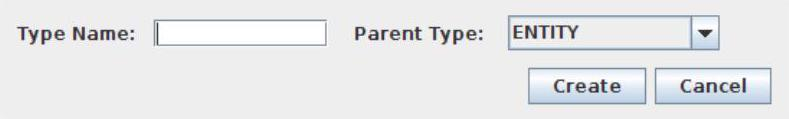
\includegraphics[max width=\textwidth]{2023_06_06_402e2c8ca4c84733095bg-3}
\end{center}

You can then enter a name for the type and choose the parent of the type. Finally click the "Create" button to finish creating the type.

Note that currently the interface only allows choosing one parent, while SNePS itself allows choosing more than one. This will be changed in a future release.

\subsection{Switching Contexts}
To switch contexts, select the appropriate context from the context tree on the right side of the main interface panel.

\begin{center}
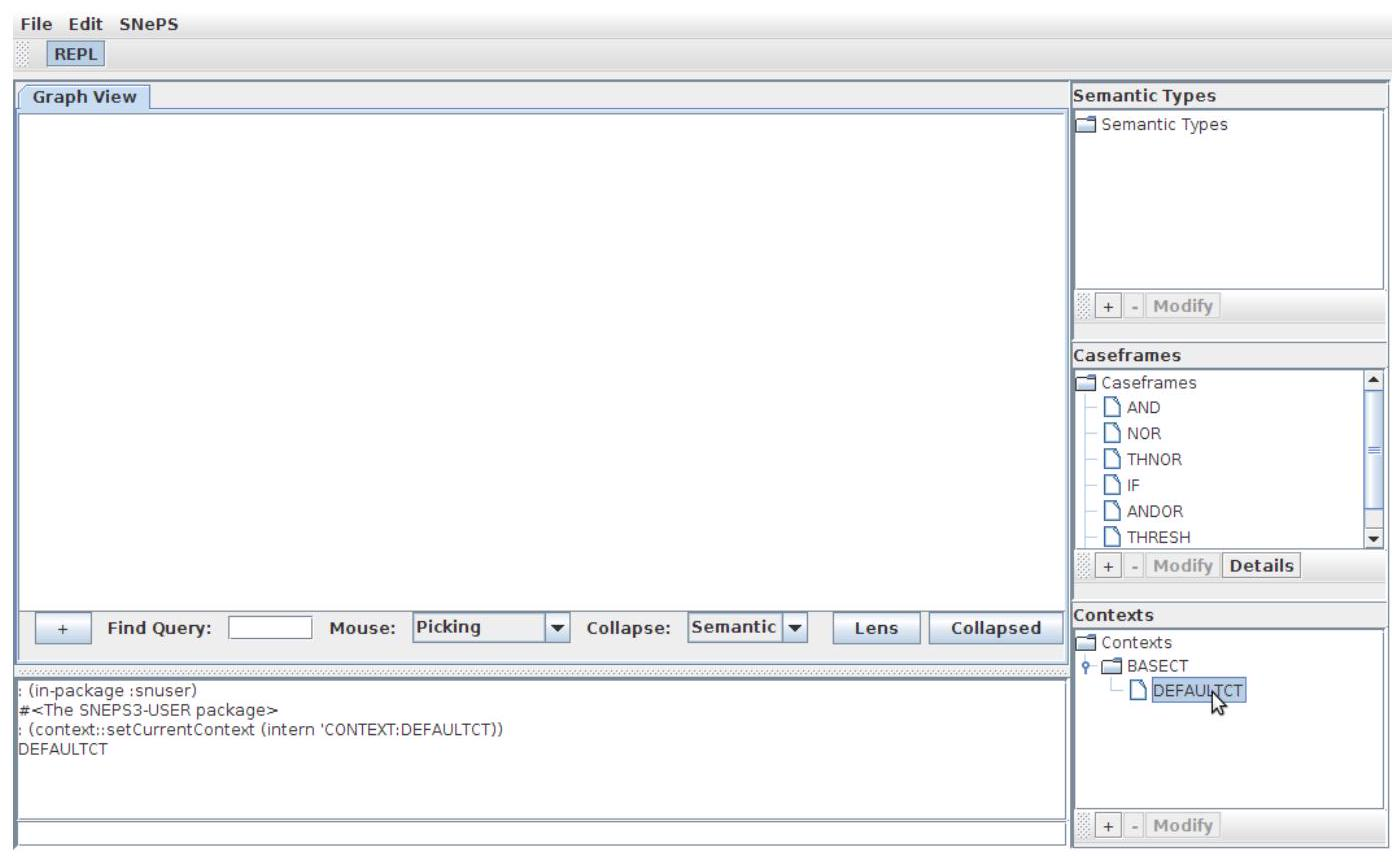
\includegraphics[max width=\textwidth]{2023_06_06_402e2c8ca4c84733095bg-3(1)}
\end{center}

\subsection{Adding a Context}
To create a context, click the "+" button under the Contexts tree on the right side of the main user interface panel. The "Define Context" window then appears.

\begin{center}
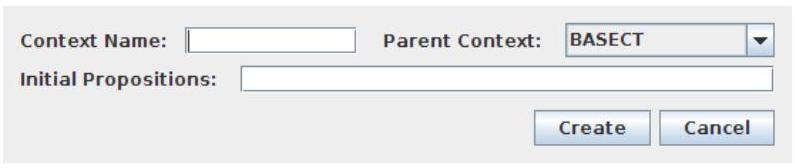
\includegraphics[max width=\textwidth]{2023_06_06_402e2c8ca4c84733095bg-4(1)}
\end{center}

Fill in a new context name, the parent of the context, and a space delimited set of assertions to be included in this context. When you have completed this, click "Create."

\subsection{Adding Slots and Caseframes}
To create a casefreame, click the "+" button under the Caseframes tree on the right side of the main user interface panel. The "Define Casefreame" window then appears.

\begin{center}
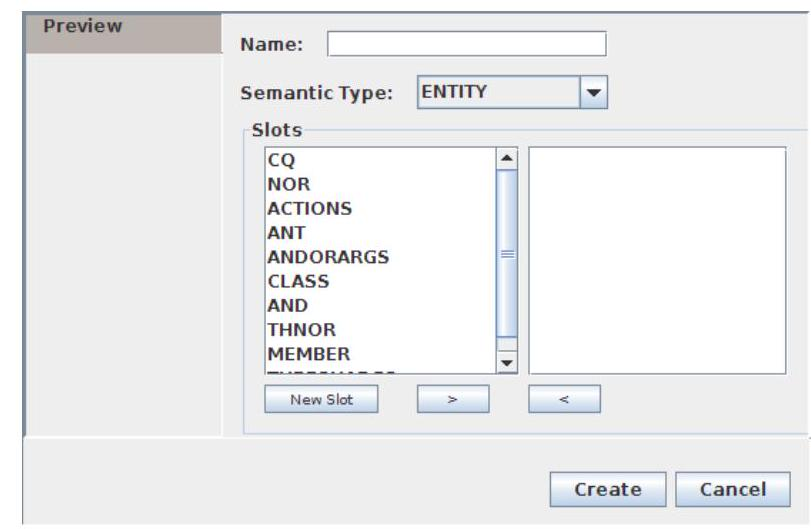
\includegraphics[max width=\textwidth]{2023_06_06_402e2c8ca4c84733095bg-4}
\end{center}

To create a caseframe enter an appropriate name for the caseframe, and select the appropriate semantic type. Next, add the slots which will be in this caseframe by selecting them in the left list and clicking the ">" button. Slots which have been added to the right list are added to the caseframe, while those in the left list are those which will not been added. You may remove an item from the right pane by selecting it and clicking the "<" button.

Note that the order of the slots in the right pane is important. The order in which the slots are added from the left selection box to the right box is the order they will be in the SNePS defineCaseframe statement. The area this will most affect the user is if these are added backwards in a binary relation then the collapsed graph will have backwards directed edges.

If a slot you wish to add is not listed you will have to create it. This is done by clicking the "New Slot" button. The Define Slot window will appear.

\begin{center}
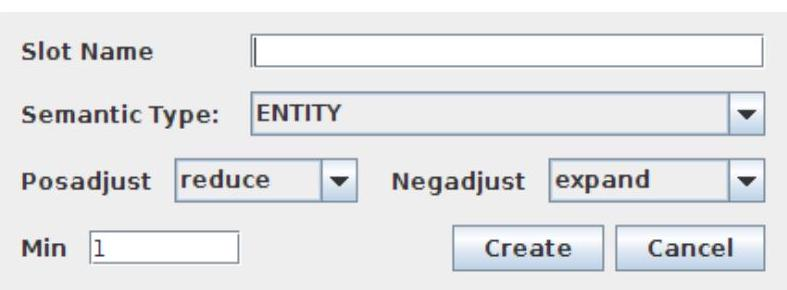
\includegraphics[max width=\textwidth]{2023_06_06_402e2c8ca4c84733095bg-5}
\end{center}

Fill in the appropriate values and click "Create." (See the SNePS 3 user manual for a description of what these options do, if needed.) The new slot will be added to the left selection list of the Define Caseframe window.

Note that after creating a caseframe you are able to see which slots are part of it by selecting it in the caseframe tree in the main user interface and clicking the "Details" button.

\subsection{Interacting with SNePS Directly}
If you wish to perform operations not supported by the user interface, or you find the interface cumbersome, you may use the REPL provided to interact with SNePS directly. Simply enter the command you wish into the REPL text box and press Enter. Note that the output displayed here is only the value returned by a command, not anything which uses the lisp format command.

\section{Using the Graph View}
The graph is created automatically when terms are added to the SNePS knowledge base. This section will assist you in manipulating the graph.

\subsection{Adding Nodes to the Graph}
When adding nodes to the graph the user adds an instance of a caseframe. To do this, click the "+" button under the graph visualization, a new window will appear.

\begin{center}
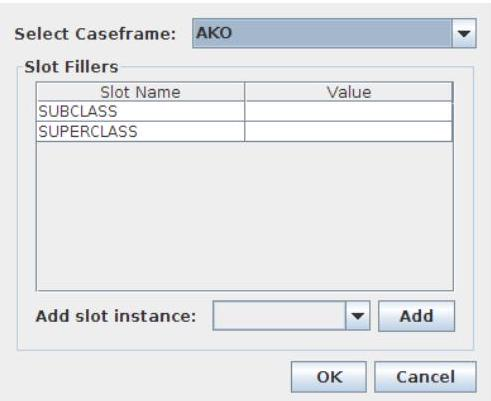
\includegraphics[max width=\textwidth]{2023_06_06_402e2c8ca4c84733095bg-5(1)}
\end{center}

First, select the caseframe which you wish to add to the graph. A list of fillers required for this caseframe appears. Double-click the value field of each filler to enter the value you wish. If you are working with a caseframe which has slots which allow for more than one filler, you may add those fillers by selecting it from the "Add slot instance" drop down and clicking "Add." When you are done, click "OK" to add the assertion to the Knowledge Base and to the graph.

\subsection{Basic Graph Manipulation}
The JUNG graph visualization toolkit which is in use here defines two modes for dealing with the graph - picking and transforming. These two options are selectable from the "Mouse" drop down box under the graph visualization window. Picking means the ability to select a single node and move it, while in the transforming mode clicking and dragging movies the entire graph.

Also, the user may zoom in to or out from the graph using the mouse wheel.

\subsection{Collapsing the Graph}
To collapse nodes using the "Semantic Collapse" method which eliminates WFT nodes from binary relations and draws arcs labeled with the relation name, click the "Collapsed" button under the graph visualization pane. In order to return to the expanded view click this button again.

\begin{center}
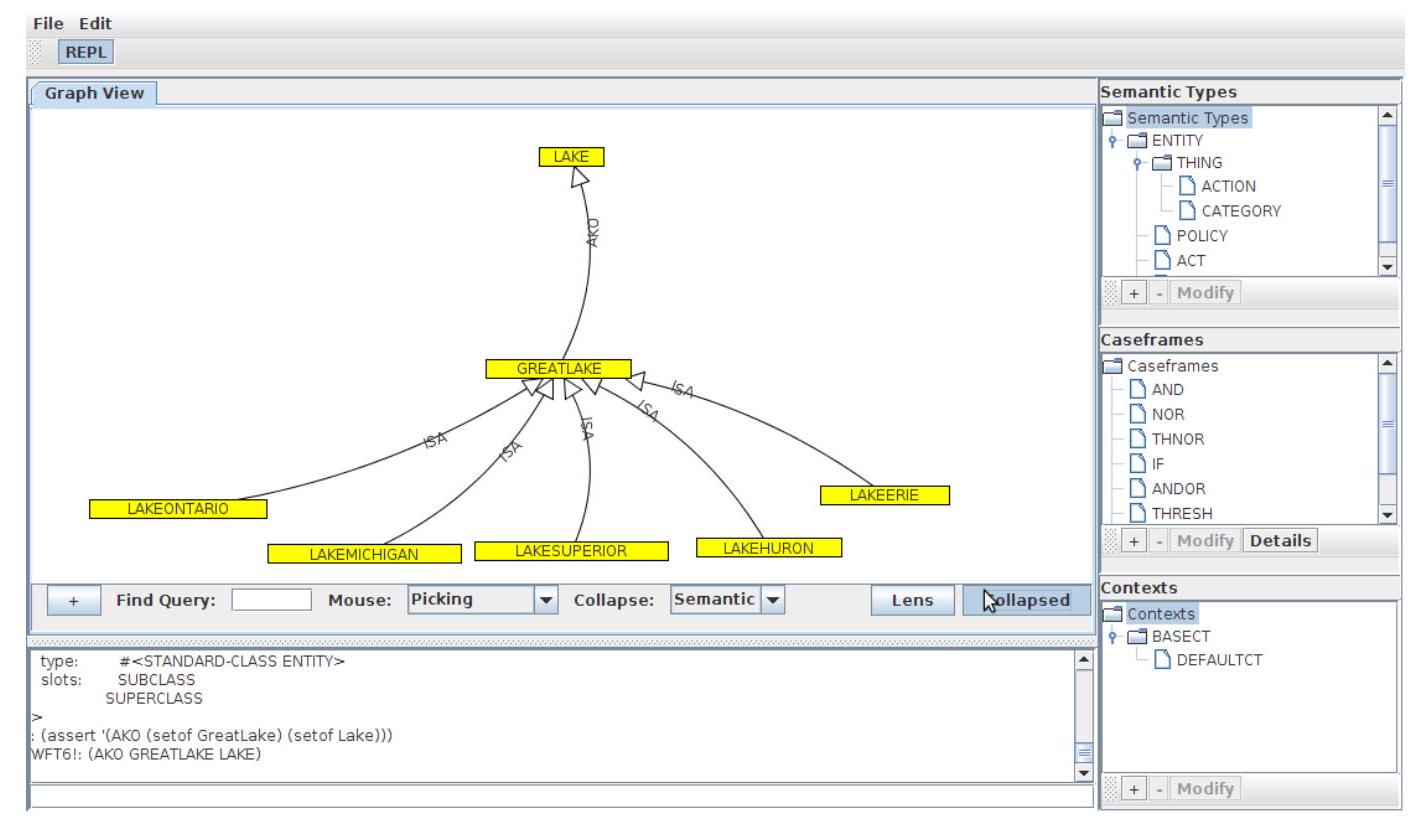
\includegraphics[max width=\textwidth]{2023_06_06_402e2c8ca4c84733095bg-6}
\end{center}

\subsection{Using a Hyperbolic Lens}
As a method to selectively zoom into a tightly clustered place in the graph you may activate a hyperbolic lens. To do this, click the "Lens" button under the graph visualization window.

\begin{center}
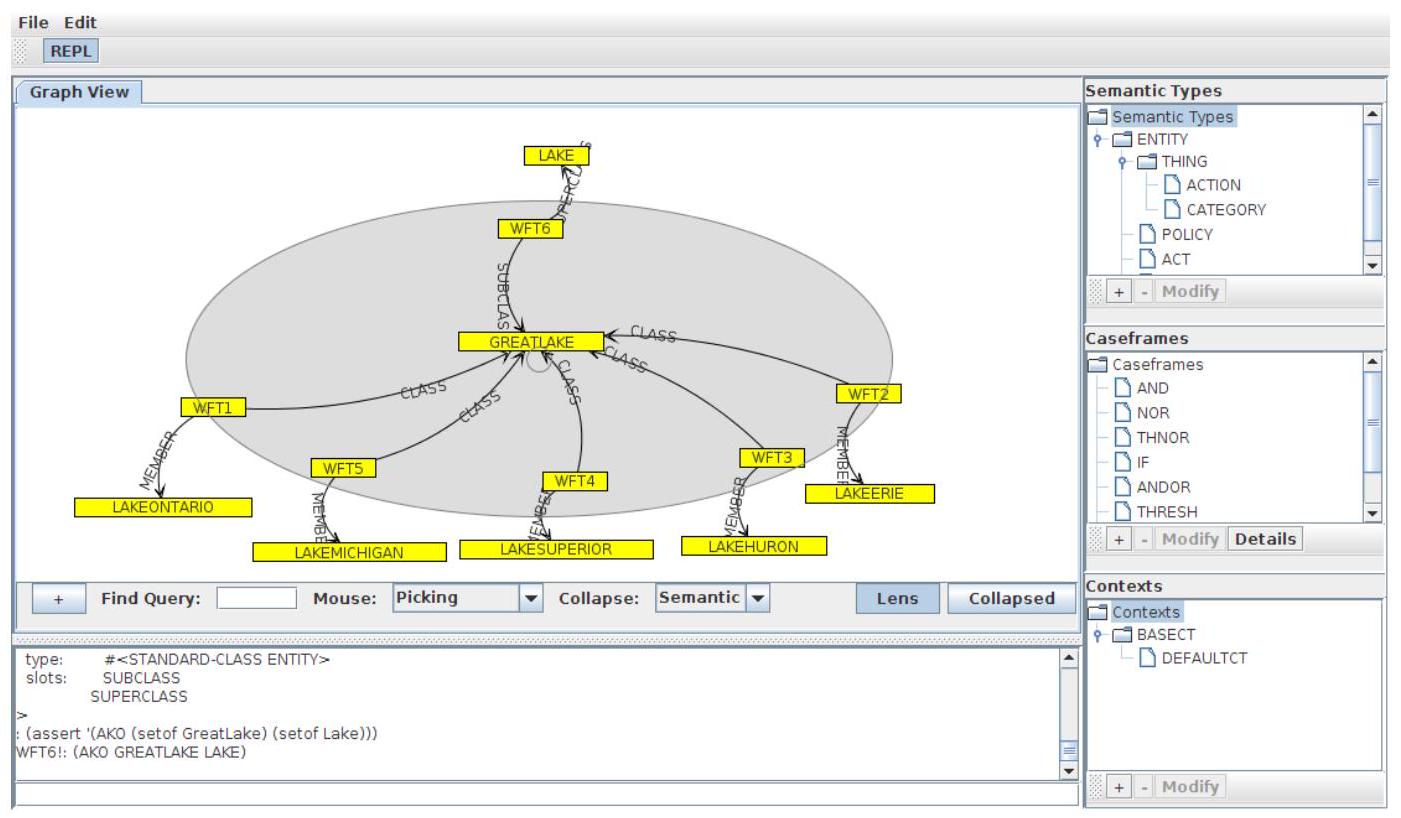
\includegraphics[max width=\textwidth]{2023_06_06_402e2c8ca4c84733095bg-7(1)}
\end{center}

The lens can be dragged when the graph is in Transforming mode. It can also be resized by clicking and dragging its edge when in this mode. To disable the lens, click the button used to activate it again.

\subsection{Using a Find Query}
You can use the find function in SNePS 3 to find a set of nodes of a certain type. In order to do this click in the text box next to the word "Find" under the graph visualization panel. The find window appears.

\begin{center}
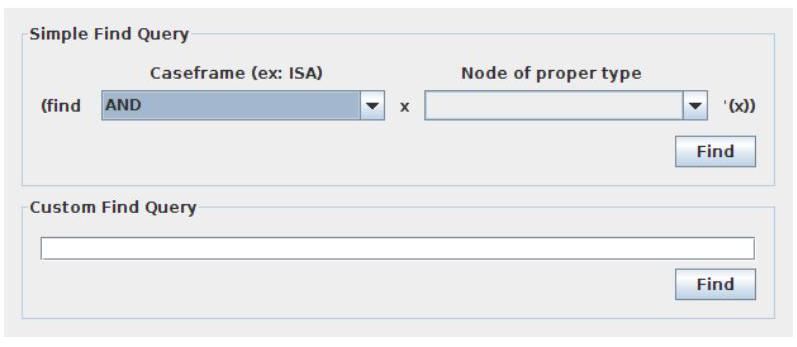
\includegraphics[max width=\textwidth]{2023_06_06_402e2c8ca4c84733095bg-7}
\end{center}

Two options are presented in this window. A simple find query can be used to find all assertions which have the selected caseframe, then a variable, and a node of a type. Alternatively the user can enter a custom find query.

The results of this are then displayed in the graph area, hiding all of the nodes which are not relevant. To exit the find mode click the "Exit Find Mode" button at the top of the graph area.

Note that this area will be redesigned in a future release to be more user friendly.


\end{document}